\documentclass[xcolor=dvipsnames,table]{beamer}

\usepackage{latexsym}
\usepackage[utf8]{inputenc}
\usepackage[brazil]{babel}
\usepackage{amssymb}
\usepackage{amsmath}
\usepackage{stmaryrd}
\usepackage{fancybox}
\usepackage{datetime}
\usepackage[T1]{fontenc}
\usepackage{graphicx}
\usepackage{graphics}
\usepackage{url}
\usepackage{algorithmic}
\usepackage{algorithm}
\usepackage{acronym}
\usepackage{array}

\newtheorem{definicao}{Definio}
\newcommand{\tab}{\hspace*{2em}}

\mode<presentation>
{
  \definecolor{colortexto}{RGB}{0,0,0}
 
  \setbeamertemplate{background canvas}[vertical shading][ bottom=white!10,top=white!10]
  \setbeamercolor{normal text}{fg=colortexto} 

  \usetheme{Warsaw}
}

\title{Caminhos e circuitos em grafos \\Cortes} 

\author{
  Esdras Lins Bispo Jr. \\ \url{bispojr@ufg.br}
  } 
 \institute{
  Teoria de Grafos \\Bacharelado em Ciência da Computação}
\date{\textbf{28 de junho de 2017} }

\logo{
\includegraphics[width=1cm]{images/ufgJataiLogo.png}}

\begin{document}

	\begin{frame}
		\titlepage
	\end{frame}

	\AtBeginSection{
		\begin{frame}{Sumário}%[allowframebreaks]{Sumário}
    		\tableofcontents[currentsection]
    		%\tableofcontents[currentsection, hideothersubsections]
		\end{frame}
	}

	\begin{frame}{Plano de Aula}
		\tableofcontents
		%\tableofcontents[hideallsubsections]
	\end{frame}
    
   \begin{frame}{Pensamento}
   	\begin{columns}
   		\column{.4\textwidth}  		
   		\begin{center}
   			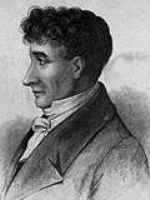
\includegraphics[width=.9\textwidth]{images/joubert.jpg}
   		\end{center}
   		\column{.6\textwidth}  		
   		\begin{block}{Frase}
   			\begin{center}
   				{\large Jamais corte o que pode ser desatado.}
   			\end{center}
   		\end{block}		  		
   		\begin{block}{Quem?}
   			\begin{center}
   				{\bf Joseph Joubert (1754 - 1824)} \\Moralista e ensaísta francês.
   			\end{center}
   		\end{block}
   	\end{columns}
   \end{frame}
    
    \section{Revisão}
	\subsection{União e Intersecção de Grafos}
	\begin{frame}{União e Intersecção de Grafos}
		\begin{block}{União}
			A {\bf união} de dois grafos $G$ e $H$ é o grafo $(V_G \cup V_H, E_G \cup E_H)$. \\É natural denotar esse grafo por $G \cup H$.
		\end{block}  
		\begin{block}{Intersecção}
			A {\bf intersecção} de dois grafos $G$ e $H$ é o grafo $(V_G \cap V_H, E_G \cap E_H)$. É natural denotar esse grafo por $G \cap H$.
		\end{block}  
		\begin{alertblock}{Alguns cuidados...}
			Para evitar grafos sem vértices, só trataremos da \\interação $G \cap H$ se $V_G \cap V_H$ não for vazio.
		\end{alertblock}
	\end{frame}
	
	\begin{frame}{União e Intersecção de Grafos}
		\begin{block}{Grafos disjuntos}
			Dois grafos $G$ e $H$ são {\bf disjuntos} se \\os conjuntos $V_G$ e $V_H$ são disjuntos.
		\end{block}  
		\begin{block}{Corolário}
			Se $G$ e $H$ são disjuntos, então $E_G$ e $E_H$ são disjuntos.
		\end{block}
	\end{frame}

	\subsection{Subgrafos}
	\begin{frame}{Subgrafos}
		\begin{block}{Definição}
			Um {\bf subgrafo} de um grafo $G$ é qualquer grafo $H$ tal que \\$V_H \subseteq V_G$ e $E_H \subseteq E_G$.
		\end{block}  
		\begin{block}{Notações e Nomenclaturas}
			\begin{itemize}
				\item É conveniente escrever ``$H \subseteq G$'' para dizer que \\$H$ é subgrafo de $G$;  
				\item Um subgrafo $H$ de $G$ é {\bf gerador} ({\it abrangente}, para alguns) \\se $V_H = V_G$;  
				\item Um subgrafo $H$ de $G$ é {\bf próprio} \\se $V_H \not= V_G$ ou $E_H \not= E_G$ (notação: $H \subset G$).
			\end{itemize}
		\end{block}
	\end{frame}
	
	\section{Subgrafos (cont.)}
	\begin{frame}{Subgrafos}
		\begin{block}{Subgrafo induzido - $G[X]$}
			O subgrafo de $G$ {\bf induzido} por um subconjunto $X$ de $V_G$ é \\o grafo $(X, F)$ em que $F$ é o conjunto $E_G \cap X^{(2)}$. \\Esse subgrafo é denotado por $G[X]$.
		\end{block} \pause
		\begin{block}{$G - X$}
			Para qualquer subconjunto $X$ de $V_G$, \\denotaremos por $G - X$ o subgrafo $G[V_G \setminus X]$.
		\end{block} \pause
		\begin{block}{$G - v$}
			Uma abreviação para $G - \{ v \}$.
		\end{block}
	\end{frame}
	
	\begin{frame}{Subgrafos}
		\begin{block}{$G - a$}
			Uma abreviação para o grafo $(V_G, E_G \setminus \{ a \})$.
		\end{block} \pause
		\begin{block}{$G - A$}
			Se $A$ é um subconjunto de $E_G$, então $G - A$ é uma abreviação para o grafo $(V_G, E_G \setminus A)$.
		\end{block} \pause
		\begin{block}{Corolário}
			$G - A$ é um grafo gerador de $G$.
		\end{block}
	\end{frame}

	\section{Caminhos e circuitos em grafos}
	\begin{frame}{Caminhos e circuitos em grafos}
		\begin{block}{Caminho em um grafo}
			Se um caminho $v_1 \ldots v_p$ é subgrafo de $G$, dizemos simplesmente que $v_1 \ldots v_p$ {\bf é um} caminho em $G$ ou que \\$G$ {\bf contém} o caminho $v_1 \ldots v_p$.
		\end{block} \pause
		\begin{exampleblock}{Circuitos em um grafo}
			Aplica-se identicamente a circuitos.
		\end{exampleblock} 
	\end{frame}
	
	\begin{frame}{Caminhos e circuitos em grafos}
		\begin{block}{Nomenclatura}
			Se $v$ e $w$ são os dois extremos de um caminho em $G$, é cômodo dizer que o caminho vai de $v$ a $w$ ou que começa em $v$ e termina em $w$.
		\end{block} \pause
		\begin{alertblock}{Cuidado!}
			Use estas expressões com cautela pois caminhos são objetos estáticos e não têm orientação.
		\end{alertblock}
	\end{frame}
	
	\begin{frame}{Caminhos e circuitos em grafos}
		\begin{block}{Caminho máximo em $G$}
			Um caminho $P$ em um grafo $G$ é máximo se $G$ não contém um caminho de comprimento maior que o de $P$.
		\end{block} \pause
		\begin{block}{Caminho maximal em $G$}
			Um caminho $P$ em $G$ é maximal se não existe caminho $P'$ em $G$ tal que $P \subset P'$.
		\end{block} \pause
		\begin{block}{Caminho Hamiltoniano}
			Um caminho é {\bf hamiltoniano} se contém todos os vértices do grafo.
		\end{block}
	\end{frame}	
	
	\section{Cortes}
	\begin{frame}{Cortes}
		\begin{block}{Definição}
			\begin{itemize}
				\item Suponha que $X$ é um conjunto de vértices de um grafo $G$. \pause
				\item O {\bf corte} associado a $X$ (ou {\bf franja} de $X$) é o conjunto de todas as arestas que têm uma ponta em $X$ e outra em $V_G \setminus X$.
			\end{itemize}
		\end{block} \pause
		\begin{block}{Notação}
			O corte associado a $X$ será denotado por
			\begin{center}
				$\partial_G (X)$
			\end{center}
		\end{block} \pause
		\begin{alertblock}{Outros autores...}
			Alguns preferem escrever $\delta(X)$ ou $\nabla(X)$.
		\end{alertblock}
	\end{frame}
	
	\begin{frame}{Cortes}
		\begin{block}{Cortes triviais}
			\begin{itemize}
				\item $\partial( \emptyset )$; \pause
				\item $\partial( V_G )$.
			\end{itemize}
		\end{block} \pause
		\begin{block}{Corolário}
			$|\partial(\{v\})| = d(v)$
		\end{block} \pause
		\begin{block}{Grau de um conjunto}
			\begin{itemize}
				\item Diremos que $|\partial(X)|$ é o {\bf grau} de $X$; \pause
				\item Denotamos este número como se segue:
				\begin{center}
					$d(X) := |\partial(X)|$
				\end{center}
			\end{itemize}
		\end{block}
	\end{frame}
	
	\begin{frame}{Cortes}
		\begin{block}{Corte - Definição}
			Um {\bf corte} ({\it = cut = coboundary}) em um grafo $G$ é qualquer conjunto da forma $\partial(X)$, em que $X$ é um subconjunto de $V_G$.
		\end{block} \pause
		\begin{alertblock}{Cuidado}
			Um corte é um conjunto de arestas, não de vértices.
		\end{alertblock}
	\end{frame}
	
	\begin{frame}
		\titlepage
	\end{frame}
	
\end{document}